\begin{frame}{Größenordnungen}
	\begin{itemize}
		\item Ein paar Zahlen im Jahr 2007 (\textbf{nur} Züge):
		\begin{itemize}
			\item 56,994 Züge, 8916 Stationen
		\end{itemize}
	\end{itemize}
	
	\begin{center}
		\begin{tabular}{ c||c|c } 
			& Time Dependent & Time Expanded \\
 			\hline
 			\hline
 			Knoten & 240 Tsd. & 3479 Tsd. \\
 			Kanten & 670 Tsd. & 5633 Tsd. \\
 			\hline
		\end{tabular}
	\end{center}
\end{frame}


\begin{frame}{Performanz}
	\begin{itemize}
		\item TD ist besser für Single-Criteria Suche\footnote{Pyrga et al.: Experimental Comparison of Shortest Path Approaches for Timetable Information, 2004}.
	\end{itemize}

	% SEHR simple annahmen, z.b. ohne Berücksichtigung von Umstiegszeiten, etc.
		\begin{center}
		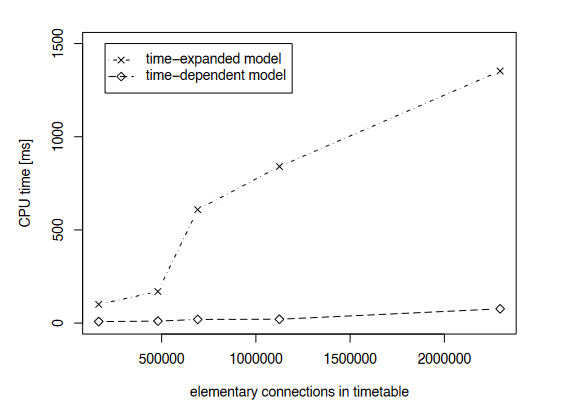
\includegraphics[height=5cm]{images/comparisons/comparison-simple.png} 
	\end{center}
\end{frame}


\begin{frame}{Performanz}
	\begin{itemize}
		\item Aber: Komplexität von TD wächst schnell mit mehr Kriteria und Regeln
		\item Also in realistischen Szenarien!
		\begin{itemize}
			\item TD nur $58\%$ schneller (in CPU-Zeit) als TE
		\end{itemize}
	\end{itemize}

\end{frame}

